\documentclass{beamer}
\mode<presentation>
{
  \usetheme{default}      % or try Darmstadt, Madrid, Warsaw, ...
  \usecolortheme{default} % or try albatross, beaver, crane, ...
  \usefonttheme{default}  % or try serif, structurebold, ...
  \setbeamertemplate{navigation symbols}{}
  \setbeamertemplate{caption}[numbered]
} 

\usepackage[english]{babel}
\usepackage[utf8]{inputenc}
\usepackage{scrextend}
\usepackage{graphicx}
\usepackage{booktabs}
\usepackage{adjustbox}
\usepackage{marvosym}
\usepackage{amsmath}
\usepackage{float}

\usepackage{booktabs, chemformula}
\usepackage{listings}
\usepackage{xcolor} 
\usepackage{array}
\usepackage{color, colortbl}
\usepackage{caption}
\captionsetup{font=footnotesize}



\definecolor{lightgreen}{rgb}{0.82, 0.94, 0.75}
\definecolor{lightorange}{rgb}{0.98, 0.84, 0.65}
\newcolumntype{L}{>{\centering\arraybackslash}m{10cm}}
\newcolumntype{l}{>{\centering\arraybackslash}m{7cm}}

\graphicspath{ {./images} }


\newcommand*{\Comb}[2]{{}^{#1}C_{#2}}%

\title[Pres]{Methods and Tools for the Analysis of Legacy Software
Systems\\
Report 2. Logical dependencies in practice.
 }
\author{Stana Adelina Diana}
\institute{Computer Science and Engineering Department\\
"Politehnica" University of Timisoara}
\date{May, 2021}

\begin{document}

\begin{frame}
  \titlepage
\end{frame}

%%%%%%%%%%%%%%%%%%%%%%%%%%%%%%%%%%%%%%%%%%
\section{Presentation of the research topic}
 \begin{frame}
\frametitle{Presentation of the research topic}
The goal of the thesis is to develop methods for analyzing legacy software systems by using historical information extracted from the versioning systems.
We divided our work into two main parts

\begin{itemize}
\item historical information collection and filtering
\item \textbf{usage of the collected information in order to analyze the software systems}
\end{itemize}

\end{frame}

%%%%%%%%%%%%%%%%%%%%%%%%%%%%%%%%%%%%%%%%%%

 \begin{frame}
\frametitle{State of the art in key classes detection}
\begin{block}{Definition}
 Classes that can be found in documents written to provide an architectural overview of the system or an introduction to the system structure. Also known as important classes.
\end{block}

\end{frame}

%%%%%%%%%%%%%%%%%%%%%%%%%%%%%%%%%%%%%%%%%%

 \begin{frame}
\frametitle{State of the art in key classes detection (cont.)}
 The key class identification can be done by using different algorithms:
\begin{itemize}
\item Osman et al., used a machine learning algorithm and class diagrams  \cite{6676885}
\item Thung et al. builds on top of Osman et al.’s approach and adds network metrics and optimistic classification \cite{rocclasification}
\item Zaidman et al. use a webmining algorithm and dynamic analysis of the source code \cite{ZaidmanJurnal}
\item Sora et al. use static analysis of the source code and a page ranking algorithm together with other class attributes \cite{Finding-key-classes}
\end{itemize}

\end{frame}

%%%%%%%%%%%%%%%%%%%%%%%%%%%%%%%%%%%%%%%%%%

 \begin{frame}
\frametitle{Results evaluation}
 To evaluate the quality of the approach and solution produced,
the key classes found are compared with a reference solution.
\textit{The reference solution is extracted from the developer's documentation.}
\end{frame}

%%%%%%%%%%%%%%%%%%%%%%%%%%%%%%%%%%%%%%%%%%

 \begin{frame}
\frametitle{Metrics for results evaluation}
For the comparison between both solutions is used a classification model and the Receiver Operating Characteristic Area Under Curve (ROC-AUC) metric to evaluate the performance.
\vskip 0.3cm
 This tool presents the result as
a number between 0 and 1. For a classifier to be considered good, its ROC-AUC metric value should be as close to 1 as possible.
\end{frame}

%%%%%%%%%%%%%%%%%%%%%%%%%%%%%%%%%%%%%%%%%%

 \begin{frame}
\frametitle{Baseline approach}
We took the research done by Sora et al. \cite{Finding-key-classes} as the baseline for our research.
 \begin{figure}[H]
\centering
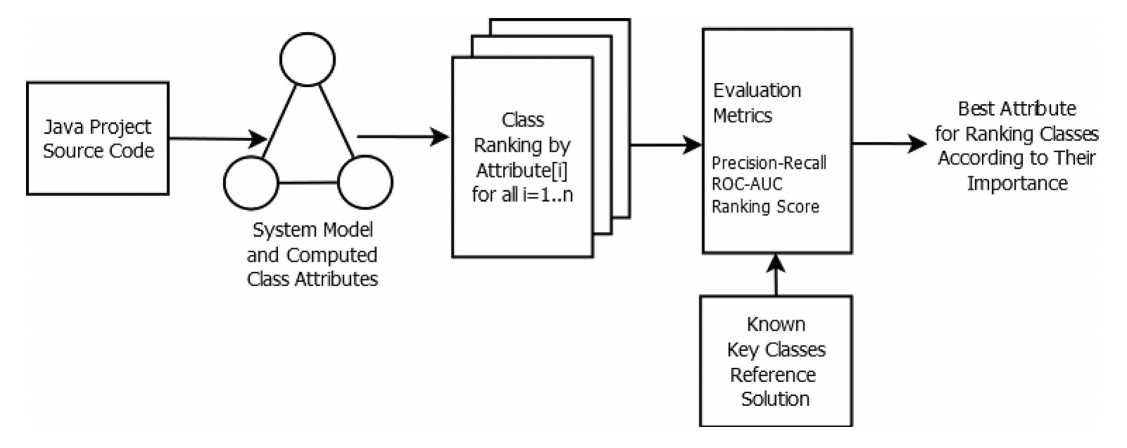
\includegraphics[width=\textwidth]{baseline_approach.PNG}
\caption{Overview of the baseline approach. From “Finding key classes in object-oriented
software systems by techniques based on static analysis.” by Ioana Sora and Ciprian-Bogdan Chirila, 2019, Information and Software Technology, 116:106176.  }
\label{fig:baseline_approach}
\centering
\end{figure}

\end{frame}

%%%%%%%%%%%%%%%%%%%%%%%%%%%%%%%%%%%%%%%%%%

 \begin{frame}
\frametitle{Data set used}
Highlighted with green are the systems used in the baseline research that can also be used in the current research.
\begin{center}
 \begin{table}[H]
\renewcommand{\arraystretch}{1}
\captionsetup{font=scriptsize}
\caption{Found systems and versions of the systems in GitHub. }
\label{tab:gitfoundsystems}
\centering
\scalebox{0.8}{
\begin{tabular}{|c|c|c|c|c|}
\hline
ID	&	System	&	Version	&	Release Tag name	&	Commits number	\\
\hline
\rowcolor{lightgreen}
Sl	&	Apache Ant	&	1.6.1	&	rel/1.6.1	&	6713	\\
S2	&	Argo UML	&	0.9.5	&	not found	&	0	\\
S3	&	GWT Portlets	&	0.9.5 beta	&	not found	&	0	\\
\rowcolor{lightgreen}
S4	&	Hibernate 	&	5.2.12	&	5.2.12	&	6733	\\
S5	&	javaclient	&	2.0.0	&	not found	&	0	\\
S6	&	jEdit	&	5.1.0	&	not found	&	0	\\
S7	&	JGAP	&	3.6.3	&	not found	&	0	\\
S8	&	JHotDraw	&	6.0b.1	&	not found	&	149	\\
S9	&	JMeter	&	2.0.1	&	v2\_1\_1	&	2506	\\
S10	&	Log4j	&	2.10.0	&	v1\_2\_10-recalled	&	634	\\
S11	&	Mars	&	3.06.0	&	not found	&	0	\\
S12	&	Maze	&	1.0.0	&	not found	&	0	\\
S13	&	Neuroph	&	2.2.0	&	not found	&	0	\\
\rowcolor{lightgreen}
S14	&	Tomcat Catalina	&	9.0.4	&	9.0.4	&	19108	\\
S15	&	Wro4J	&	1.6.3	&	v1.6.3	&	2871	\\
\hline
\end{tabular}
}
\end{table}
\end{center}
\end{frame}

%%%%%%%%%%%%%%%%%%%%%%%%%%%%%%%%%%%%%%%%%%

 \begin{frame}
\frametitle{Comparison with the baseline approach}
 \begin{center}
     \begin{figure}
	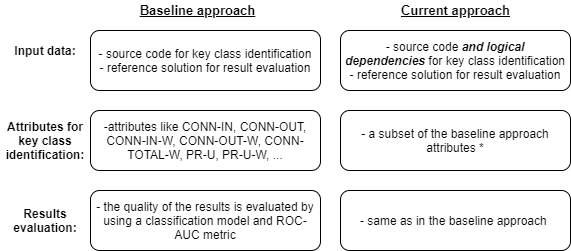
\includegraphics[width=\textwidth]{baseline_comparison.png}
	\caption{\label{fig:fig}Comparison between the new approach and the baselines}
     \end{figure}
\end{center}

\textit{* The reason why we are not using all the attributes is that the extracted logical dependencies are undirected.}
\end{frame}

%%%%%%%%%%%%%%%%%%%%%%%%%%%%%%%%%%%%%%%%%%

 \begin{frame}
\frametitle{Logical dependencies collection}
Two filters are applied to co-changing pairs: the commit size filter with threshold 10, and the connection strength filter with a variable threshold. 
 \begin{center}
     \begin{figure}
	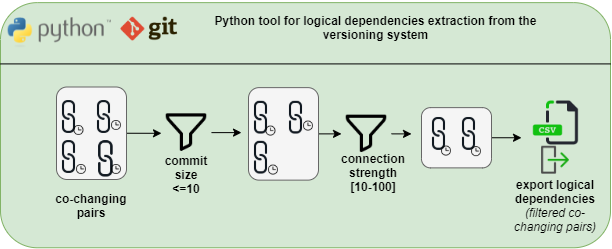
\includegraphics[width=\textwidth]{ld_collection.png}
	\caption{\label{fig:fig}Logical dependencies extraction workflow and filters used}
     \end{figure}
\end{center}
\end{frame}

%%%%%%%%%%%%%%%%%%%%%%%%%%%%%%%%%%%%%%%%%%

 \begin{frame}
\frametitle{Current workflow}
We couple the tool that extracts logical dependencies and the tool that identifies key classes and evaluates the results.
 \begin{center}
     \begin{figure}
	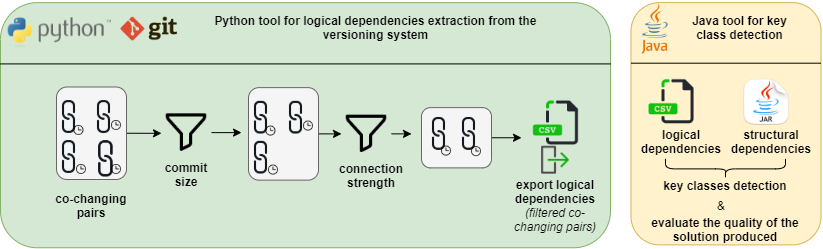
\includegraphics[scale=0.4]{key_class_workflow.png}
	\caption{\label{fig:fig}Workflow for key classes detection and evaluation of results}
     \end{figure}
\end{center}
\end{frame}

%%%%%%%%%%%%%%%%%%%%%%%%%%%%%%%%%%%%%%%%%%

 \begin{frame}
\frametitle{Measurements using only the baseline approach}
In table are presented the ROC-AUC values for different attributes computed for the systems Ant, Tomcat Catalina, and Hibernate by using the baseline approach.
  \begin{center}
\begin{table}[!h]
\renewcommand{\arraystretch}{1}
\caption{ROC-AUC metric values extracted. }
\label{tab:previousresults}
\centering
\scalebox{0.9}{
\begin{tabular}{|c|ccc|}
\hline
Metrics &	Ant	&	Tomcat Catalina	&	Hibernate	\\
\hline

PR\_U2\_W	&	0.95823	&	0.92341	&	0.95823	\\
PR	&	0.94944	&	0.92670	&	0.94944	\\
PR\_U	&	0.95060	&	0.93220	&	0.95060	\\
CONN\_TOTAL\_W	&	0.94437	&	0.92595	&	0.94437	\\
CONN\_TOTAL	&	0.94630	&	0.93903	&	0.94630	\\

\hline
\end{tabular}
}
\end{table}
\end{center}
\end{frame}

%%%%%%%%%%%%%%%%%%%%%%%%%%%%%%%%%%%%%%%%%%

 \begin{frame}
\frametitle{Measurements using combined SD and LD}
The tool used by the baseline approach builds a graph that contains the structural dependencies extracted from static source code analysis.
We modified the tool to read also logical dependencies and add them to the graph. 

\begin{table}[!h]
\renewcommand{\arraystretch}{1}
\caption{Measurements for Ant using structural and logical dependencies combined}
\label{tab:measurementscombined:ant}
\centering
\scalebox{0.6}{
\begin{tabular}{|c|cccccccccc|c|}
\hline
Metrics &	$\geq10\%$	&	$\geq20\%$		&	$\geq30\%$		&	$\geq40\%$		&	$\geq50\%$		&	$\geq60\%$		&	$\geq70\%$		&	$\geq80\%$		&	$\geq90\%$		&	$\geq100\%$		&	Baseline \\
\hline

PR\_U2\_W	&	0.924	&	0.925	&	0.926	&	0.927	&	0.927	&	0.927	&	\cellcolor{lightgreen}0.929	&	0.928	&	0.928	&	0.928	&	0.929	\\
PR	&	0.914	&	0.854	&	0.851	&	\cellcolor{lightgreen}0.866	&	\cellcolor{lightgreen}0.876	&	\cellcolor{lightgreen}0.882	&	\cellcolor{lightgreen}0.887	&	0.854	&	0.852	&	0.852	&	0.855	\\
PR\_U	&	0.910	&	0.930	&	0.933	&	0.933	&	\cellcolor{lightgreen}0.935	&	\cellcolor{lightgreen}0.934	&	\cellcolor{lightgreen}0.939	&	0.933	&	0.933	&	0.933	&	0.933	\\
CON\_T\_W	&	0.924	&	0.928	&	0.931	&	0.932	&	0.933	&	0.934	&	\cellcolor{lightgreen}0.936	&	0.934	&	0.934	&	0.934	&	0.934	\\
CON\_T	&	0.840	&	0.886	&	0.904	&	0.909	&	0.915	&	0.923	&	0.932	&	0.935	&	\cellcolor{lightorange}0.936	&	\cellcolor{lightorange}0.936	&	0.942	\\

\hline
\end{tabular}
}
\end{table}
\end{frame}

%%%%%%%%%%%%%%%%%%%%%%%%%%%%%%%%%%%%%%%%%%

 \begin{frame}
\frametitle{Measurements using combined SD and LD (cont.)}
 \begin{center}
     \begin{figure}
	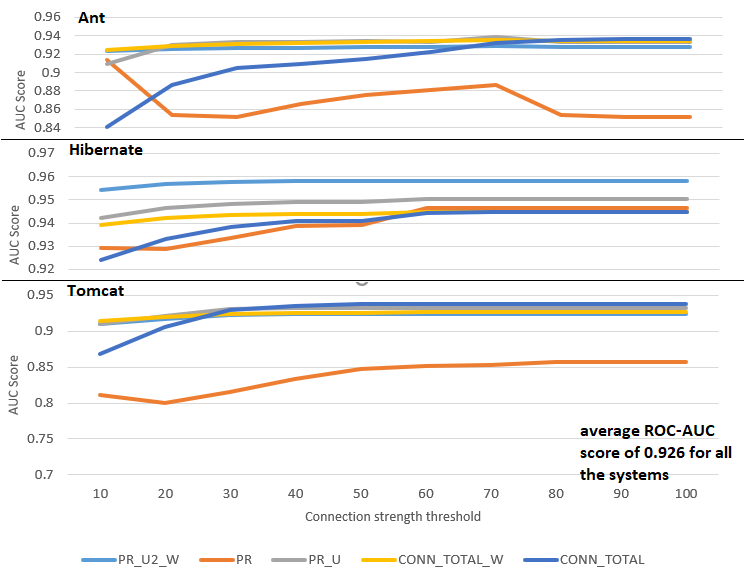
\includegraphics[width=\textwidth]{ld_st_measurements.png}
     \end{figure}
\end{center}

\end{frame}


%%%%%%%%%%%%%%%%%%%%%%%%%%%%%%%%%%%%%%%%%%

 \begin{frame}
\frametitle{Measurements using only logical dependencies}
For this type of measurement, we add only the logical dependencies to the graph.

\begin{table}[!h]
\renewcommand{\arraystretch}{1}
\caption{Measurements for Ant using only logical dependencies}
\label{tab:measurementshistory:ant}
\centering
\scalebox{0.6}{
\begin{tabular}{|c|cccccccccc|c|}
\hline
Metrics &	$\geq10\%$	&	$\geq20\%$		&	$\geq30\%$		&	$\geq40\%$		&	$\geq50\%$		&	$\geq60\%$		&	$\geq70\%$		&	$\geq80\%$		&	$\geq90\%$		&	$\geq100\%$		&	Baseline \\
\hline

PR\_U2\_W	&	0.720	&	0.627	&	0.718	&	0.703	&	0.732	&	0.824	&	0.852	&	\cellcolor{lightorange}0.881	&	0.876	&	0.876	&	0.929	\\
PR	&	0.720	&	0.627	&	0.718	&	0.703	&	0.732	&	0.824	&	0.852	&	\cellcolor{lightorange}0.881	&	0.876	&	0.876	&	0.855	\\
PR\_U	&	0.720	&	0.627	&	0.718	&	0.703	&	0.732	&	0.824	&	0.852	&	\cellcolor{lightorange}0.881	&	0.876	&	0.876	&	0.933	\\
CON\_T\_W	&	0.722	&	0.581	&	0.644	&	0.676	&	0.727	&	0.819	&	0.842	&	0.874	&	\cellcolor{lightorange}0.876	&	0.876	&	0.934	\\
CON\_T	&	0.722	&	0.581	&	0.644	&	0.676	&	0.727	&	0.819	&	0.842	&	0.874	&	\cellcolor{lightorange}0.876	&	0.876	&	0.942	\\

\hline
\end{tabular}
}
\end{table}

\end{frame}


%%%%%%%%%%%%%%%%%%%%%%%%%%%%%%%%%%%%%%%%%%

 \begin{frame}
\frametitle{Measurements using only logical dependencies (cont.) }
 \begin{center}
     \begin{figure}
	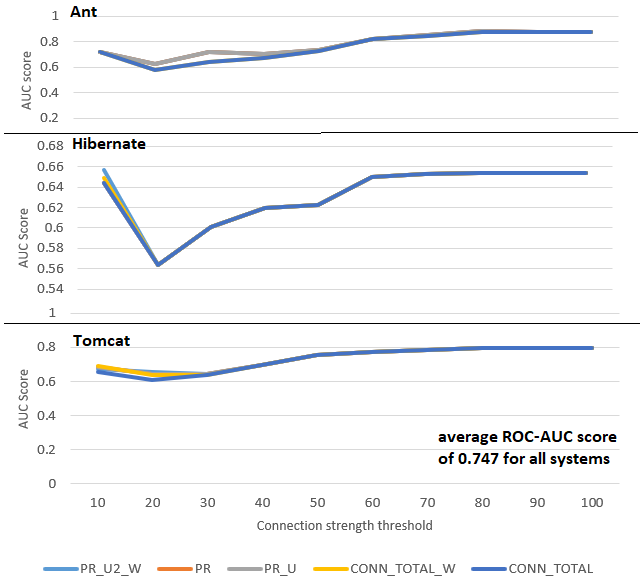
\includegraphics[scale=0.68]{ld_measurements.png}
     \end{figure}
\end{center}
\end{frame}

%%%%%%%%%%%%%%%%%%%%%%%%%%%%%%%%%%%%%%%%%%

 \begin{frame}
\frametitle{Comparison with fan-in and fan-out metric}
\begin{block}{Definition}


\begin{itemize}
\item The fan-in of entity A is the total number of entities that call functions of A.
\item The fan-out of A is the total number of entities called by A.
\end{itemize}

\end{block}
\end{frame}


%%%%%%%%%%%%%%%%%%%%%%%%%%%%%%%%%%%%%%%%%%

 \begin{frame}
\frametitle{Comparison with fan-in and fan-out metric (cont.)}
By looking at the comparisons between FAN IN, FAN OUT, FAN TOTAL, and the logical dependencies in which a class is involved we could not determine a direct connection between them.

\begin{table}[!h]
\renewcommand{\arraystretch}{1}
\caption{Top 10 LD measurements for Ant. }
\label{tab:measurementstop:ant}
\centering
\scalebox{0.7}{
\begin{tabular}{|c|ccccc|}
\hline
Nr.	&	Classname	&	FAN\_IN	&	FAN\_OUT	&	FAN\_TOTAL	&	LD\_NUMBER \\
\hline
1	&	\cellcolor{lightorange}Project	&	191	&	23	&	214	&	157	\\
2	&	Project\$AntRefTable	&	1	&	2	&	3	&	157	\\
3	&	Path	&	39	&	13	&	52	&	147	\\
4	&	Path\$PathElement	&	3	&	2	&	5	&	147	\\
5	&	\cellcolor{lightorange}IntrospectionHelper	&	18	&	24	&	42	&	143	\\
6	&	IntrospectionHelper\$AttributeSetter	&	8	&	1	&	9	&	143	\\
7	&	IntrospectionHelper\$Creator	&	3	&	5	&	8	&	143	\\
8	&	IntrospectionHelper\$NestedCreator	&	7	&	1	&	8	&	143	\\
9	&	Ant	&	2	&	15	&	17	&	136	\\
10	&	Ant\$Reference	&	3	&	1	&	4	&	136	\\
\hline
\end{tabular}
}
\end{table}

\end{frame}

%%%%%%%%%%%%%%%%%%%%%%%%%%%%%%%%%%%%%%%%%%

 \begin{frame}
\frametitle{Conclusions}
 The advantage of using \textit{only logical dependencies} in key class detection is that it only uses data extracted from the versioning system
and can be generalized to various programming languages.

\begin{itemize}
\item by using both dependencies combined, we can obtain a slightly better ROC-AUC score than the one obtained by the baseline approach
\item by using only logical dependencies we obtain comparable  results with the ones obtained by other researchers
\end{itemize}

\begin{table}[!h]
\renewcommand{\arraystretch}{1}
\label{tab:measurementstop:ant}
\centering
\scalebox{0.7}{
\begin{tabular}{|c|ccccc|}
\hline
	&	Thung et al.	&	 Osman et al.	& Baseline  &	Current approach  & Current approach\\
	&		&		&  &	 (SD+LD) &  (LD) \\
\hline
 ROC-AUC score & 	0.825	&	0.750 & 	0.894	&	 0.926 & 0.747	\\
\hline
\end{tabular}
}
\end{table}



\begin{itemize}
\item the logical dependencies number can be used complementary with fan-in and fan-out metric.
\end{itemize}



\end{frame}

\begin{frame}
\bibliographystyle{plain}
\footnotesize
\bibliography{logicaldepd}
\end{frame}

\end{document}
